\section{Resistive Circuits}

\subsection{Resistors in Series and Parallel}
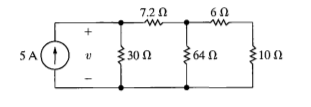
\includegraphics[scale=0.5]{img/c3/p1}
For the circuit shown above, find:
\begin{enumerate}
	\item The voltage $v$
	\item The power delivered to the circuit by the current source
	\item The power dissipated in the $10 \Omega$ resistor
\end{enumerate}

We begin by starting from the farthest right side of the circuit. Then, by alternating combing
series and parallel resistor we can reduce down to one resistor. 
\begin{enumerate}
	\item First combine the $6\Omega$ and $10\Omega$ in series to get $16\Omega$
	\item Now combine that in parallel with the $64_\Omega$ $\frac{(16)(64)}{16+63} = 12.8\Omega$
	\item Now comine that in series with the $7.2\Omega$ resistor to get $20 \Omega$
	\item Then combine that in parallel with the $30\Omega$ $\frac{(20)(30)}{20+30} = 12\Omega$
\end{enumerate} 
This gives us the below circuit:
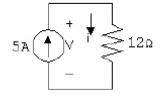
\includegraphics{img/c3/a1}

With the simplified circuit the problem becomes easier. 
1) Using Ohm's Law we can see that:
\\$ V = IR = (5 A)(12 \Omega) = 60 V$\\
2) Now that we know the value of the voltage drop accross the current source we can find the power:
\\$ p = -(V)(I) = -(60 V)(5 A) = -300 W$ \\
Therefore 300 W is delivered to the circuit.
3) Now we know that the voltage drop across the current source is 60 V. This is also the voltage drop
across the $30 \Omega$ resistor. Therefore the current through this resistor is:
\\ $i_A = \frac{60 V}{30 \Omega} = 2 A $ \\
Using KCL in the upper left node, we can solve for $i_B$
\begin{align*}
	0 &= -5 A + i_A + i_B \\
	i_B &= 5A - i_A \\
	i_B &= 5A - 2A \\
	i_B &= 3A \\
\end{align*}
Next, we can create a KVL equation of the outer loop of the circuit. and solve for $i_C$
\begin{align*}
	0 &= -v + 7.2i_B + 6i_C \\
	16i_C &= v - 7.2i_B \\
	16i_C &= 60V - (7.2)(3) \\
	i_c &= \frac{38.4}{16} \\
	i_c &= 2.4 A
\end{align*}

Now that we know the current through the $10 \Omega$ resistor, we can use that to find the power:
\\$ p_{10\Omega} = (10)(2.4)^2 = 57.6W $\\

\subsection{The Voltage-Divider and Current-Divider Circuits}

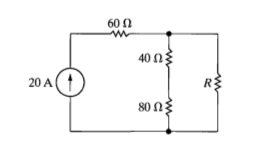
\includegraphics{img/c3/p2}
\\In the above Circuit:
\begin{enumerate}
	\item Find the value of R that will cause 4A of current to flow through the $80 \Omega$
	resistor in the crcuit shown. 
	\item How much power will the resistor $R$ from part 1 need to dissipate?
	\item How much power will the current source generate for the value of $R$ from part 1?
\end{enumerate}

1) The current will be divided between the branch with $R$ and the branch with the $40\Omega$ and
$80\Omega$ resistors. Therefore:
\begin{align*}
	i_{80\Omega} &= \frac{R}{R+40\Omega+80\Omega} \times (20A) \\
	i_{80\Omega} &= 4 A \\
	4 A &= \frac{R}{R+40\Omega+80\Omega} \times (20A) \\
	20R &= 4(R+120) \\
	16R &= 480 \\
	R &= \frac{480}{16} \\
	R &= 30\Omega
\end{align*}

2) With $R = 30\Omega$ we can then calculate the current through R usin gcurrent division, then
solve for the power. 
\begin{align*}
	i_R &= \frac{40+80}{40+80+30}(20 A) \\
	i_R &= 16 A \\
	p_R &= (30)(16)^2 \\
	p_R &= 7680 W
\end{align*}

3) Finally, we can make a KVL equation around the outer loop to solve for the voltage $v$, then solve for power:

\begin{align*}
	0 &= -v + (60 \Omega)(20 A) + (30 \Omega)(16 A) \\
	v &= 1200 + 480 \\
	v &= 1680 V \\
	p_{source} &= -vi \\
	p_{source} &= -(1680 V)(20 A) \\
	p_{source} &= -33,600 W
\end{align*}




\subsection{Voltage and Current Divisions}
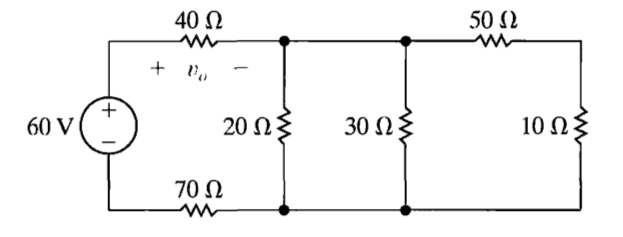
\includegraphics[scale=0.5]{img/c3/p3}
Using the above circuit, answer the following questions:
\begin{enumerate}
	\item Use voltage division to determine the voltage $v_o$ across the $40 \Omega$ resistor.
	\item Use $v_o$ from part 1 to determine the current through the $40 \Omega$ resistor. Use
	this current and current division to calculate the current in the $30 \Omega$ resistor.
	\item How much power is abosrbed by the $50 \Omega$ resistor?
\end{enumerate}

1) First we need to find the equivalent resistance of all the resistors to the right of the $40 \Omega$
and $70 \Omega$ Resistors. 
\\$R_{eq} = 20\Omega \parallel 30\Omega \parallel (50 \Omega + 10 \Omega) $\\
\\$ \frac{1}{R_{eq}} = \frac{1}{20} \frac{1}{30} + \frac{1}{60} = \frac{1}{10} $\\
Therefore $R_{eq} = 10 \Omega$ and the voltage is:
\\$ v_o = \frac{40}{40+10+70}(60 V) = 20 V $\\


2) First we can find the current through the $40\Omega$ resistor:
\\ $ i_{40\Omega} = \frac{v_o}{40} = \frac{20 V}{40\Omega} = 0.5 A $ \\

Then we will need to find the equivalent circuit of the two parallel branches in order to use
current division. 
\\ $20 \Omega \parallel(50 \Omega + 10 \Omega) = \frac{(20)(60)}{(20+60)} = 15 \Omega $ \\
\\ $i_{30 \Omega} = \frac{15}{15+30} \times 0.5A = 0.16667 A = 166.67 mA $ \\

3) We can find the power dissipated by the $50 \Omega$ resistor by fnding the current through it. 
We use current division to find the current in the $40 \Omega$ resistor, but first the equivalent 
resistance of the $20 \Omega$ and $30 \Omega$ branches must be calculated:
\\$ 20 \Omega \parallel 30\Omega = \frac{(20(30)}{20+30} = 12 \Omega $\\
Then current division gives:
\\$ i_{50\Omega} = \frac{12}{12+50+10} \times 0.5A = 0.08333A $\\
Thus:
\\ $p_{50\Omega} = (50)(0.083333)^2 = 0.034722 W = 347.22 mW $ \\


\subsection{Delta-Wye Equivalent Circuits}
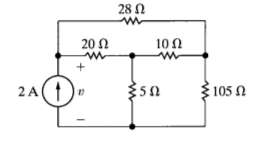
\includegraphics{img/c3/p4}

Use a Y to $\Delta$ transformation to find the voltage $v$ in the circuit shown. 

First we can convert the three Y-connected resistors (20 10, and 5 $\Omega$) to three
$\Delta$-connected resistors as shown below. Not that this diagram shows the old and new resistors
to help with visualization. \\
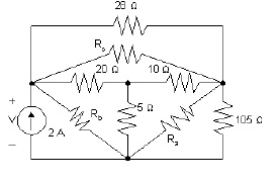
\includegraphics{img/c3/a4}
\\ Then we can solve for the new resistors:

\begin{align*}
	R_a &= \frac{(5)(10) + (5)(20) + (10)(20)}{20} = 17.5 \Omega \\
	R_b &= \frac{(5)(10) + (5)(20) + (10)(20)}{10} = 35 \Omega \\
	R_c &= \frac{(5)(10) + (5)(20) + (10)(20)}{5} = 70 \Omega \\
\end{align*}

This gives us the following circuit: \\
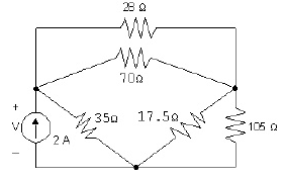
\includegraphics{img/c3/a5}
\\From this circuit we can see the $70 \Omega$ resistor is in parallel with the $28 \Omega$ Resistor 
and that the $17.5 \Omega$ resistor is in parallel with the $105 \Omega$ resistor. 
\\ $ 70 \Omega \parallel 28 \Omega = \frac{(70)(28)}{70+28} = 20 \Omega $\\
\\ $ 17.5 \Omega \parallel 105 \Omega = \frac{(17.5)(105)}{17.5+105} = 15 \Omega $\\

Now we can see that the equivalent $20 \Omega$ resistor is in series with the equivalent $15 \Omega$
reistor, giving a $35 \Omega$ equivalent resistance. Putting this resistor in parallel with the
other $35 \Omega$ resistor means: 
\\ $ 35 \Omega \parallel 35 \Omega = \frac{(35)(35)}{35+35} = 17.5 \Omega  $ \\
This means the resistance seen by the 2 A source is $17.5 \Omega$. Therefore:
\\$ v = ir = (17.5 \Omega)(2 A) = 35 V $\\

